% Plot a graph using TikZ/PGFPlots
%
% pgfplot.tex is created by the PGFPlot output of the ModelleertaalApp.
%
\documentclass[12pt]{standalone}
\usepackage{tikz}
\usepackage{pgfplots}
\usepackage{helvet}
\usepackage[detect-none, list-final-separator={ en }, per-mode=symbol,
            retain-explicit-plus, output-decimal-marker={,},
            exponent-product={\cdot}, range-phrase={ tot }]{siunitx}
\usepackage[font={small,sf},labelfont={bf},labelsep=endash]{caption}
\usepackage[eulergreek]{sansmath}
\pgfplotsset{
  tick label style = {font=\sansmath\sffamily},
  every axis label = {font=\sansmath\sffamily},
  legend style = {font=\sansmath\sffamily},
  label style = {font=\sansmath\sffamily},
  /pgf/number format/.cd,
  use comma,
  1000 sep={},
}
\begin{document}

% Use \input{} to wrap this inside suitable LaTeX doc:
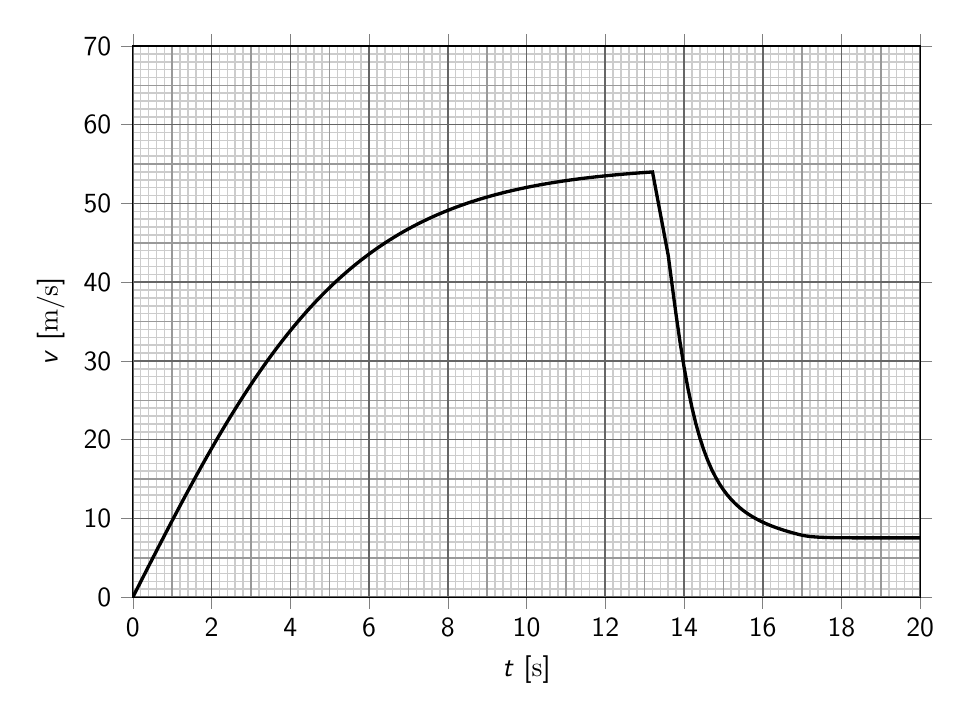
\begin{tikzpicture}
% draw 10x10cm millimeter paper.
\def\width{10}
\def\height{7}
\draw[step=1mm, line width=0.2mm, black!20!white] (0,0) grid (\width,\height);
\draw[step=5mm, line width=0.2mm, black!40!white] (0,0) grid (\width,\height);
\draw[step=1cm, line width=0.2mm, black!60!white] (0,0) grid (\width,\height);
%
%
%
%x and y scale set to 10cmx10cm grid. Adjust to fit!
% x = [0 .. 99.8999999999986]
% y = [0 .. 54.0000612508191]
% this only works for graphs starting a (0,0)
\begin{axis}[x=1cm/2, y=1cm/10,
enlargelimits=false, tick align=outside,
 xlabel={$t$ [\si{\second}]},
ylabel={$v$ [\si{\meter\per\second}]},
% xtick={0, 1, 2, ..., 10},
% ytick={0, 2, 4, ..., 20},
xmin=0, xmax=20, ymin=0, ymax=70]
\addplot[no marks, black, very thick]
coordinates {
(0,0)
(0.1,0.9810000000000001)
(0.2,1.96168696829011)
(0.30000000000000004,2.941435240965471)
(0.4,3.919620950616096)
(0.5,4.895623615665144)
(0.6,5.868827713848075)
(0.7,6.838624231358504)
(0.7999999999999999,7.804412179393882)
(0.8999999999999999,8.76560007011707)
(0.9999999999999999,9.721607344404529)
(1.0999999999999999,10.671865744173541)
(1.2,11.615820622564032)
(1.3,12.552932185788501)
(1.4000000000000001,13.482676661049537)
(1.5000000000000002,14.404547385550485)
(1.6000000000000003,15.318055812283188)
(1.7000000000000004,16.22273242895902)
(1.8000000000000005,17.118127587147335)
(1.9000000000000006,18.003812239390633)
(2.0000000000000004,18.879378582770013)
(2.1000000000000005,19.744440608090034)
(2.2000000000000006,20.598634554531557)
(2.3000000000000007,21.441619270277386)
(2.400000000000001,22.273076480242516)
(2.500000000000001,23.0927109626328)
(2.600000000000001,23.90025063660786)
(2.700000000000001,24.69544656383222)
(2.800000000000001,25.478072867159497)
(2.9000000000000012,26.24792657010544)
(3.0000000000000013,27.004827361125248)
(3.1000000000000014,27.748617287017513)
(3.2000000000000015,28.47916038003175)
(3.3000000000000016,29.196342223458494)
(3.4000000000000017,29.90006946063226)
(3.5000000000000018,30.590269252379308)
(3.600000000000002,31.266888687996687)
(3.700000000000002,31.929894154858925)
(3.800000000000002,32.57927067171696)
(3.900000000000002,33.21502119068367)
(4.000000000000002,33.83716587279523)
(4.100000000000001,34.44574134190105)
(4.200000000000001,35.04079992147075)
(4.300000000000001,35.62240885871864)
(4.4,36.19064954023763)
(4.5,36.74561670310937)
(4.6,37.28741764521928)
(4.699999999999999,37.816171438256525)
(4.799999999999999,38.33200814662434)
(4.899999999999999,38.83506805522692)
(4.999999999999998,39.32550090883921)
(5.099999999999998,39.80346516550689)
(5.1999999999999975,40.26912726616866)
(5.299999999999997,40.72266092244278)
(5.399999999999997,41.164246424277)
(5.4999999999999964,41.594069968926604)
(5.599999999999996,42.012323012500595)
(5.699999999999996,42.419201645102376)
(5.799999999999995,42.81490599038861)
(5.899999999999995,43.19963963017995)
(5.999999999999995,43.573609054579386)
(6.099999999999994,43.93702313788902)
(6.199999999999994,44.29009264046381)
(6.299999999999994,44.633029736501335)
(6.399999999999993,44.96604756763981)
(6.499999999999993,45.28935982212206)
(6.5999999999999925,45.603180339180405)
(6.699999999999992,45.90772273820661)
(6.799999999999992,46.2032000721908)
(6.8999999999999915,46.489824504843966)
(6.999999999999991,46.76780701075892)
(7.099999999999991,47.037357097914644)
(7.19999999999999,47.298682551787174)
(7.29999999999999,47.55198920029719)
(7.39999999999999,47.79748069879837)
(7.499999999999989,48.03535833429178)
(7.599999999999989,48.26582084803911)
(7.699999999999989,48.489064275740255)
(7.799999999999988,48.70528180443947)
(7.899999999999988,48.91466364532699)
(7.999999999999988,49.11739692160996)
(8.099999999999987,49.31366557063735)
(8.199999999999987,49.50365025947718)
(8.299999999999986,49.68752831316098)
(8.399999999999986,49.86547365482926)
(8.499999999999986,50.03765675703271)
(8.599999999999985,50.20424460346628)
(8.699999999999985,50.36540066043707)
(8.799999999999985,50.521284857391834)
(8.899999999999984,50.67205357585562)
(8.999999999999984,50.817859646158986)
(9.099999999999984,50.95885235135795)
(9.199999999999983,51.09517743777731)
(9.299999999999983,51.22697713163468)
(9.399999999999983,51.35439016122883)
(9.499999999999982,51.47755178420225)
(9.599999999999982,51.59659381941347)
(9.699999999999982,51.711644682979845)
(9.799999999999981,51.82282942807616)
(9.89999999999998,51.93026978809845)
(9.99999999999998,52.03408422282554)
(10.09999999999998,52.13438796723346)
(10.19999999999998,52.23129308263947)
(10.29999999999998,52.324908509873495)
(10.399999999999979,52.41534012419468)
(10.499999999999979,52.5026907916901)
(10.599999999999978,52.587060426911115)
(10.699999999999978,52.66854605152023)
(10.799999999999978,52.747241853738245)
(10.899999999999977,52.823239248397236)
(10.999999999999977,52.89662693742004)
(11.099999999999977,52.967490970561194)
(11.199999999999976,53.035914806257814)
(11.299999999999976,53.10197937245161)
(11.399999999999975,53.16576312725535)
(11.499999999999975,53.22734211934831)
(11.599999999999975,53.28679004799591)
(11.699999999999974,53.34417832259889)
(11.799999999999974,53.39957612168646)
(11.899999999999974,53.45305045127675)
(11.999999999999973,53.50466620253628)
(12.099999999999973,53.554486208677304)
(12.199999999999973,53.60257130103959)
(12.299999999999972,53.64898036430928)
(12.399999999999972,53.69377039083402)
(12.499999999999972,53.73699653399891)
(12.599999999999971,53.7787121606335)
(12.69999999999997,53.81896890242443)
(12.79999999999997,53.857816706313265)
(12.89999999999997,53.89530388386297)
(12.99999999999997,53.93147715958028)
(13.09999999999997,53.966381718184856)
(13.199999999999969,54.0000612508191)
(13.599999999999968,43.37324133185011)
(13.699999999999967,39.535377676549395)
(13.799999999999967,35.813498347957065)
(13.899999999999967,32.36175333913768)
(13.999999999999966,29.25489674874352)
(14.099999999999966,26.512483422607684)
(14.199999999999966,24.121051752933123)
(14.299999999999965,22.050346937451994)
(14.399999999999965,20.263645614022156)
(14.499999999999964,18.7236479561547)
(14.599999999999964,17.395475970704833)
(14.699999999999964,16.247949441290096)
(14.799999999999963,15.253912274250466)
(14.899999999999963,14.39007768829127)
(14.999999999999963,13.636659459676222)
(15.099999999999962,12.976933475380868)
(15.199999999999962,12.396802520158065)
(15.299999999999962,11.884397528271757)
(15.399999999999961,11.429727344049311)
(15.499999999999961,11.024378323436737)
(15.59999999999996,10.661260151022026)
(15.69999999999996,10.334392346066682)
(15.79999999999996,10.038725579432572)
(15.89999999999996,9.76999229694955)
(15.99999999999996,9.52458180579697)
(16.09999999999996,9.299435705684024)
(16.19999999999996,9.091960230322977)
(16.29999999999996,8.89995266402091)
(16.399999999999963,8.72153950263789)
(16.499999999999964,8.555124442702509)
(16.599999999999966,8.399344618649101)
(16.699999999999967,8.253033779174412)
(16.79999999999997,8.115191312205425)
(16.89999999999997,7.984956204878635)
(16.99999999999997,7.861585169263311)
(17.099999999999973,7.772076525427727)
(17.199999999999974,7.706805816662228)
(17.299999999999976,7.659034697290102)
(17.399999999999977,7.6239778549438855)
(17.49999999999998,7.5982010920871605)
(17.59999999999998,7.57922066974453)
(17.69999999999998,7.565229940170595)
(17.799999999999983,7.554909191600138)
(17.899999999999984,7.547291386210493)
(17.999999999999986,7.541666272184117)
(18.099999999999987,7.537511304274585)
(18.19999999999999,7.5344415500465605)
(18.29999999999999,7.532173184241095)
(18.39999999999999,7.530496787083305)
(18.499999999999993,7.529257759740879)
(18.599999999999994,7.528341930435727)
(18.699999999999996,7.527664959363005)
(18.799999999999997,7.527164531023965)
(18.9,7.526794595820743)
(19,7.526521120410243)
(19.1,7.526318950065386)
(19.200000000000003,7.5261694912757795)
(19.300000000000004,7.52605899973045)
(19.400000000000006,7.525977315301074)
(19.500000000000007,7.5259169271869855)
(19.60000000000001,7.525872282981356)
(19.70000000000001,7.525839277976464)
(19.80000000000001,7.5258148776693155)
(19.900000000000013,7.5257968387145695)
(20.000000000000014,7.525783502644252)
(20.100000000000016,7.525773643375533)
(20.200000000000017,7.525766354479316)
(20.30000000000002,7.525760965841382)
(20.40000000000002,7.525756982051994)
(20.50000000000002,7.525754036858501)
(20.600000000000023,7.525751859492865)
(20.700000000000024,7.525750249778021)
(20.800000000000026,7.525749059724285)
(20.900000000000027,7.525748179923747)
(21.00000000000003,7.5257475294917535)
(21.10000000000003,7.525747048630722)
(21.20000000000003,7.525746693132622)
(21.300000000000033,7.525746430314692)
(21.400000000000034,7.525746236014735)
(21.500000000000036,7.525746092369764)
(21.600000000000037,7.525745986173767)
(21.70000000000004,7.525745907663605)
(21.80000000000004,7.52574584962144)
(21.90000000000004,7.5257458067111624)
(22.000000000000043,7.525745774987811)
(22.100000000000044,7.525745751534899)
(22.200000000000045,7.5257457341962795)
(22.300000000000047,7.525745721377926)
(22.40000000000005,7.525745711901382)
(22.50000000000005,7.525745704895421)
(22.60000000000005,7.52574569971595)
(22.700000000000053,7.525745695886792)
(22.800000000000054,7.525745693055916)
(22.900000000000055,7.525745690963063)
(23.000000000000057,7.525745689415828)
(23.10000000000006,7.525745688271964)
(23.20000000000006,7.525745687426312)
(23.30000000000006,7.525745686801126)
(23.400000000000063,7.5257456863389285)
(23.500000000000064,7.5257456859972285)
(23.600000000000065,7.525745685744612)
(23.700000000000067,7.525745685557853)
(23.800000000000068,7.525745685419784)
(23.90000000000007,7.52574568531771)
(24.00000000000007,7.525745685242247)
(24.100000000000072,7.5257456851864575)
(24.200000000000074,7.525745685145212)
(24.300000000000075,7.52574568511472)
(24.400000000000077,7.525745685092177)
(24.500000000000078,7.525745685075512)
(24.60000000000008,7.525745685063191)
(24.70000000000008,7.5257456850540825)
(24.800000000000082,7.525745685047348)
(24.900000000000084,7.52574568504237)
(25.000000000000085,7.5257456850386895)
(25.100000000000087,7.525745685035968)
(25.200000000000088,7.525745685033956)
(25.30000000000009,7.5257456850324695)
(25.40000000000009,7.52574568503137)
(25.500000000000092,7.525745685030557)
(25.600000000000094,7.525745685029956)
(25.700000000000095,7.525745685029512)
(25.800000000000097,7.525745685029183)
(25.900000000000098,7.525745685028941)
(26.0000000000001,7.525745685028761)
(26.1000000000001,7.525745685028628)
(26.200000000000102,7.5257456850285305)
(26.300000000000104,7.525745685028458)
(26.400000000000105,7.525745685028404)
(26.500000000000107,7.525745685028364)
(26.600000000000108,7.525745685028335)
(26.70000000000011,7.525745685028314)
(26.80000000000011,7.525745685028298)
(26.900000000000112,7.525745685028285)
(27.000000000000114,7.5257456850282765)
(27.100000000000115,7.52574568502827)
(27.200000000000117,7.525745685028266)
(27.300000000000118,7.525745685028262)
(27.40000000000012,7.52574568502826)
(27.50000000000012,7.525745685028258)
(27.600000000000122,7.525745685028256)
(27.700000000000124,7.525745685028255)
(27.800000000000125,7.525745685028254)
(27.900000000000126,7.525745685028253)
(28.000000000000128,7.525745685028253)
(28.10000000000013,7.525745685028253)
(28.20000000000013,7.525745685028253)
(28.300000000000132,7.525745685028253)
(28.400000000000134,7.525745685028253)
(28.500000000000135,7.525745685028253)
(28.600000000000136,7.525745685028253)
(28.700000000000138,7.525745685028253)
(28.80000000000014,7.525745685028253)
(28.90000000000014,7.525745685028253)
(29.000000000000142,7.525745685028253)
(29.100000000000144,7.525745685028253)
(29.200000000000145,7.525745685028253)
(29.300000000000146,7.525745685028253)
(29.400000000000148,7.525745685028253)
(29.50000000000015,7.525745685028253)
(29.60000000000015,7.525745685028253)
(29.700000000000152,7.525745685028253)
(29.800000000000153,7.525745685028253)
(29.900000000000155,7.525745685028253)
(30.000000000000156,7.525745685028253)
(30.100000000000158,7.525745685028253)
(30.20000000000016,7.525745685028253)
(30.30000000000016,7.525745685028253)
(30.400000000000162,7.525745685028253)
(30.500000000000163,7.525745685028253)
(30.600000000000165,7.525745685028253)
(30.700000000000166,7.525745685028253)
(30.800000000000168,7.525745685028253)
(30.90000000000017,7.525745685028253)
(31.00000000000017,7.525745685028253)
(31.100000000000172,7.525745685028253)
(31.200000000000173,7.525745685028253)
(31.300000000000175,7.525745685028253)
(31.400000000000176,7.525745685028253)
(31.500000000000178,7.525745685028253)
(31.60000000000018,7.525745685028253)
(31.70000000000018,7.525745685028253)
(31.800000000000182,7.525745685028253)
(31.900000000000183,7.525745685028253)
(32.000000000000185,7.525745685028253)
(32.100000000000186,7.525745685028253)
(32.20000000000019,7.525745685028253)
(32.30000000000019,7.525745685028253)
(32.40000000000019,7.525745685028253)
(32.50000000000019,7.525745685028253)
(32.60000000000019,7.525745685028253)
(32.700000000000195,7.525745685028253)
(32.800000000000196,7.525745685028253)
(32.9000000000002,7.525745685028253)
(33.0000000000002,7.525745685028253)
(33.1000000000002,7.525745685028253)
(33.2000000000002,7.525745685028253)
(33.3000000000002,7.525745685028253)
(33.400000000000205,7.525745685028253)
(33.500000000000206,7.525745685028253)
(33.60000000000021,7.525745685028253)
(33.70000000000021,7.525745685028253)
(33.80000000000021,7.525745685028253)
(33.90000000000021,7.525745685028253)
(34.00000000000021,7.525745685028253)
(34.100000000000215,7.525745685028253)
(34.200000000000216,7.525745685028253)
(34.30000000000022,7.525745685028253)
(34.40000000000022,7.525745685028253)
(34.50000000000022,7.525745685028253)
(34.60000000000022,7.525745685028253)
(34.70000000000022,7.525745685028253)
(34.800000000000225,7.525745685028253)
(34.900000000000226,7.525745685028253)
(35.00000000000023,7.525745685028253)
(35.10000000000023,7.525745685028253)
(35.20000000000023,7.525745685028253)
(35.30000000000023,7.525745685028253)
(35.40000000000023,7.525745685028253)
(35.500000000000234,7.525745685028253)
(35.600000000000236,7.525745685028253)
(35.70000000000024,7.525745685028253)
(35.80000000000024,7.525745685028253)
(35.90000000000024,7.525745685028253)
(36.00000000000024,7.525745685028253)
(36.10000000000024,7.525745685028253)
(36.200000000000244,7.525745685028253)
(36.300000000000246,7.525745685028253)
(36.40000000000025,7.525745685028253)
(36.50000000000025,7.525745685028253)
(36.60000000000025,7.525745685028253)
(36.70000000000025,7.525745685028253)
(36.80000000000025,7.525745685028253)
(36.900000000000254,7.525745685028253)
(37.000000000000256,7.525745685028253)
(37.10000000000026,7.525745685028253)
(37.20000000000026,7.525745685028253)
(37.30000000000026,7.525745685028253)
(37.40000000000026,7.525745685028253)
(37.50000000000026,7.525745685028253)
(37.600000000000264,7.525745685028253)
(37.700000000000266,7.525745685028253)
(37.80000000000027,7.525745685028253)
(37.90000000000027,7.525745685028253)
(38.00000000000027,7.525745685028253)
(38.10000000000027,7.525745685028253)
(38.20000000000027,7.525745685028253)
(38.300000000000274,7.525745685028253)
(38.400000000000276,7.525745685028253)
(38.50000000000028,7.525745685028253)
(38.60000000000028,7.525745685028253)
(38.70000000000028,7.525745685028253)
(38.80000000000028,7.525745685028253)
(38.90000000000028,7.525745685028253)
(39.000000000000284,7.525745685028253)
(39.100000000000286,7.525745685028253)
(39.20000000000029,7.525745685028253)
(39.30000000000029,7.525745685028253)
(39.40000000000029,7.525745685028253)
(39.50000000000029,7.525745685028253)
(39.60000000000029,7.525745685028253)
(39.700000000000294,7.525745685028253)
(39.800000000000296,7.525745685028253)
(39.9000000000003,7.525745685028253)
(40.0000000000003,7.525745685028253)
(40.1000000000003,7.525745685028253)
(40.2000000000003,7.525745685028253)
(40.3000000000003,7.525745685028253)
(40.400000000000304,7.525745685028253)
(40.500000000000306,7.525745685028253)
(40.60000000000031,7.525745685028253)
(40.70000000000031,7.525745685028253)
(40.80000000000031,7.525745685028253)
(40.90000000000031,7.525745685028253)
(41.00000000000031,7.525745685028253)
(41.100000000000314,7.525745685028253)
(41.200000000000315,7.525745685028253)
(41.30000000000032,7.525745685028253)
(41.40000000000032,7.525745685028253)
(41.50000000000032,7.525745685028253)
(41.60000000000032,7.525745685028253)
(41.70000000000032,7.525745685028253)
(41.800000000000324,7.525745685028253)
(41.900000000000325,7.525745685028253)
(42.00000000000033,7.525745685028253)
(42.10000000000033,7.525745685028253)
(42.20000000000033,7.525745685028253)
(42.30000000000033,7.525745685028253)
(42.40000000000033,7.525745685028253)
(42.500000000000334,7.525745685028253)
(42.600000000000335,7.525745685028253)
(42.70000000000034,7.525745685028253)
(42.80000000000034,7.525745685028253)
(42.90000000000034,7.525745685028253)
(43.00000000000034,7.525745685028253)
(43.10000000000034,7.525745685028253)
(43.200000000000344,7.525745685028253)
(43.300000000000345,7.525745685028253)
(43.40000000000035,7.525745685028253)
(43.50000000000035,7.525745685028253)
(43.60000000000035,7.525745685028253)
(43.70000000000035,7.525745685028253)
(43.80000000000035,7.525745685028253)
(43.900000000000354,7.525745685028253)
(44.000000000000355,7.525745685028253)
(44.10000000000036,7.525745685028253)
(44.20000000000036,7.525745685028253)
(44.30000000000036,7.525745685028253)
(44.40000000000036,7.525745685028253)
(44.50000000000036,7.525745685028253)
(44.600000000000364,7.525745685028253)
(44.700000000000365,7.525745685028253)
(44.80000000000037,7.525745685028253)
(44.90000000000037,7.525745685028253)
(45.00000000000037,7.525745685028253)
(45.10000000000037,7.525745685028253)
(45.20000000000037,7.525745685028253)
(45.300000000000374,7.525745685028253)
(45.400000000000375,7.525745685028253)
(45.50000000000038,7.525745685028253)
(45.60000000000038,7.525745685028253)
(45.70000000000038,7.525745685028253)
(45.80000000000038,7.525745685028253)
(45.90000000000038,7.525745685028253)
(46.000000000000384,7.525745685028253)
(46.100000000000385,7.525745685028253)
(46.20000000000039,7.525745685028253)
(46.30000000000039,7.525745685028253)
(46.40000000000039,7.525745685028253)
(46.50000000000039,7.525745685028253)
(46.60000000000039,7.525745685028253)
(46.700000000000394,7.525745685028253)
(46.800000000000395,7.525745685028253)
(46.9000000000004,7.525745685028253)
(47.0000000000004,7.525745685028253)
(47.1000000000004,7.525745685028253)
(47.2000000000004,7.525745685028253)
(47.3000000000004,7.525745685028253)
(47.400000000000404,7.525745685028253)
(47.500000000000405,7.525745685028253)
(47.600000000000406,7.525745685028253)
(47.70000000000041,7.525745685028253)
(47.80000000000041,7.525745685028253)
(47.90000000000041,7.525745685028253)
(48.00000000000041,7.525745685028253)
(48.10000000000041,7.525745685028253)
(48.200000000000415,7.525745685028253)
(48.300000000000416,7.525745685028253)
(48.40000000000042,7.525745685028253)
(48.50000000000042,7.525745685028253)
(48.60000000000042,7.525745685028253)
(48.70000000000042,7.525745685028253)
(48.80000000000042,7.525745685028253)
(48.900000000000425,7.525745685028253)
(49.000000000000426,7.525745685028253)
(49.10000000000043,7.525745685028253)
(49.20000000000043,7.525745685028253)
(49.30000000000043,7.525745685028253)
(49.40000000000043,7.525745685028253)
(49.50000000000043,7.525745685028253)
(49.600000000000435,7.525745685028253)
(49.700000000000436,7.525745685028253)
(49.80000000000044,7.525745685028253)
(49.90000000000044,7.525745685028253)
(50.00000000000044,7.525745685028253)
(50.10000000000044,7.525745685028253)
(50.20000000000044,7.525745685028253)
(50.300000000000445,7.525745685028253)
(50.400000000000446,7.525745685028253)
(50.50000000000045,7.525745685028253)
(50.60000000000045,7.525745685028253)
(50.70000000000045,7.525745685028253)
(50.80000000000045,7.525745685028253)
(50.90000000000045,7.525745685028253)
(51.000000000000455,7.525745685028253)
(51.100000000000456,7.525745685028253)
(51.20000000000046,7.525745685028253)
(51.30000000000046,7.525745685028253)
(51.40000000000046,7.525745685028253)
(51.50000000000046,7.525745685028253)
(51.60000000000046,7.525745685028253)
(51.700000000000465,7.525745685028253)
(51.800000000000466,7.525745685028253)
(51.90000000000047,7.525745685028253)
(52.00000000000047,7.525745685028253)
(52.10000000000047,7.525745685028253)
(52.20000000000047,7.525745685028253)
(52.30000000000047,7.525745685028253)
(52.400000000000475,7.525745685028253)
(52.500000000000476,7.525745685028253)
(52.60000000000048,7.525745685028253)
(52.70000000000048,7.525745685028253)
(52.80000000000048,7.525745685028253)
(52.90000000000048,7.525745685028253)
(53.00000000000048,7.525745685028253)
(53.100000000000485,7.525745685028253)
(53.200000000000486,7.525745685028253)
(53.30000000000049,7.525745685028253)
(53.40000000000049,7.525745685028253)
(53.50000000000049,7.525745685028253)
(53.60000000000049,7.525745685028253)
(53.70000000000049,7.525745685028253)
(53.800000000000495,7.525745685028253)
(53.900000000000496,7.525745685028253)
(54.0000000000005,7.525745685028253)
(54.1000000000005,7.525745685028253)
(54.2000000000005,7.525745685028253)
(54.3000000000005,7.525745685028253)
(54.4000000000005,7.525745685028253)
(54.500000000000504,7.525745685028253)
(54.600000000000506,7.525745685028253)
(54.70000000000051,7.525745685028253)
(54.80000000000051,7.525745685028253)
(54.90000000000051,7.525745685028253)
(55.00000000000051,7.525745685028253)
(55.10000000000051,7.525745685028253)
(55.200000000000514,7.525745685028253)
(55.300000000000516,7.525745685028253)
(55.40000000000052,7.525745685028253)
(55.50000000000052,7.525745685028253)
(55.60000000000052,7.525745685028253)
(55.70000000000052,7.525745685028253)
(55.80000000000052,7.525745685028253)
(55.900000000000524,7.525745685028253)
(56.000000000000526,7.525745685028253)
(56.10000000000053,7.525745685028253)
(56.20000000000053,7.525745685028253)
(56.30000000000053,7.525745685028253)
(56.40000000000053,7.525745685028253)
(56.50000000000053,7.525745685028253)
(56.600000000000534,7.525745685028253)
(56.700000000000536,7.525745685028253)
(56.80000000000054,7.525745685028253)
(56.90000000000054,7.525745685028253)
(57.00000000000054,7.525745685028253)
(57.10000000000054,7.525745685028253)
(57.20000000000054,7.525745685028253)
(57.300000000000544,7.525745685028253)
(57.400000000000546,7.525745685028253)
(57.50000000000055,7.525745685028253)
(57.60000000000055,7.525745685028253)
(57.70000000000055,7.525745685028253)
(57.80000000000055,7.525745685028253)
(57.90000000000055,7.525745685028253)
(58.000000000000554,7.525745685028253)
(58.100000000000556,7.525745685028253)
(58.20000000000056,7.525745685028253)
(58.30000000000056,7.525745685028253)
(58.40000000000056,7.525745685028253)
(58.50000000000056,7.525745685028253)
(58.60000000000056,7.525745685028253)
(58.700000000000564,7.525745685028253)
(58.800000000000566,7.525745685028253)
(58.90000000000057,7.525745685028253)
(59.00000000000057,7.525745685028253)
(59.10000000000057,7.525745685028253)
(59.20000000000057,7.525745685028253)
(59.30000000000057,7.525745685028253)
(59.400000000000574,7.525745685028253)
(59.500000000000576,7.525745685028253)
(59.60000000000058,7.525745685028253)
(59.70000000000058,7.525745685028253)
(59.80000000000058,7.525745685028253)
(59.90000000000058,7.525745685028253)
(60.00000000000058,7.525745685028253)
(60.100000000000584,7.525745685028253)
(60.200000000000585,7.525745685028253)
(60.30000000000059,7.525745685028253)
(60.40000000000059,7.525745685028253)
(60.50000000000059,7.525745685028253)
(60.60000000000059,7.525745685028253)
(60.70000000000059,7.525745685028253)
(60.800000000000594,7.525745685028253)
(60.900000000000595,7.525745685028253)
(61.0000000000006,7.525745685028253)
(61.1000000000006,7.525745685028253)
(61.2000000000006,7.525745685028253)
(61.3000000000006,7.525745685028253)
(61.4000000000006,7.525745685028253)
(61.500000000000604,7.525745685028253)
(61.600000000000605,7.525745685028253)
(61.70000000000061,7.525745685028253)
(61.80000000000061,7.525745685028253)
(61.90000000000061,7.525745685028253)
(62.00000000000061,7.525745685028253)
(62.10000000000061,7.525745685028253)
(62.200000000000614,7.525745685028253)
(62.300000000000615,7.525745685028253)
(62.40000000000062,7.525745685028253)
(62.50000000000062,7.525745685028253)
(62.60000000000062,7.525745685028253)
(62.70000000000062,7.525745685028253)
(62.80000000000062,7.525745685028253)
(62.900000000000624,7.525745685028253)
(63.000000000000625,7.525745685028253)
(63.10000000000063,7.525745685028253)
(63.20000000000063,7.525745685028253)
(63.30000000000063,7.525745685028253)
(63.40000000000063,7.525745685028253)
(63.50000000000063,7.525745685028253)
(63.600000000000634,7.525745685028253)
(63.700000000000635,7.525745685028253)
(63.80000000000064,7.525745685028253)
(63.90000000000064,7.525745685028253)
(64.00000000000064,7.525745685028253)
(64.10000000000063,7.525745685028253)
(64.20000000000063,7.525745685028253)
(64.30000000000062,7.525745685028253)
(64.40000000000062,7.525745685028253)
(64.50000000000061,7.525745685028253)
(64.6000000000006,7.525745685028253)
(64.7000000000006,7.525745685028253)
(64.8000000000006,7.525745685028253)
(64.90000000000059,7.525745685028253)
(65.00000000000058,7.525745685028253)
(65.10000000000058,7.525745685028253)
(65.20000000000057,7.525745685028253)
(65.30000000000057,7.525745685028253)
(65.40000000000056,7.525745685028253)
(65.50000000000055,7.525745685028253)
(65.60000000000055,7.525745685028253)
(65.70000000000054,7.525745685028253)
(65.80000000000054,7.525745685028253)
(65.90000000000053,7.525745685028253)
(66.00000000000053,7.525745685028253)
(66.10000000000052,7.525745685028253)
(66.20000000000051,7.525745685028253)
(66.30000000000051,7.525745685028253)
(66.4000000000005,7.525745685028253)
(66.5000000000005,7.525745685028253)
(66.60000000000049,7.525745685028253)
(66.70000000000049,7.525745685028253)
(66.80000000000048,7.525745685028253)
(66.90000000000047,7.525745685028253)
(67.00000000000047,7.525745685028253)
(67.10000000000046,7.525745685028253)
(67.20000000000046,7.525745685028253)
(67.30000000000045,7.525745685028253)
(67.40000000000045,7.525745685028253)
(67.50000000000044,7.525745685028253)
(67.60000000000043,7.525745685028253)
(67.70000000000043,7.525745685028253)
(67.80000000000042,7.525745685028253)
(67.90000000000042,7.525745685028253)
(68.00000000000041,7.525745685028253)
(68.1000000000004,7.525745685028253)
(68.2000000000004,7.525745685028253)
(68.3000000000004,7.525745685028253)
(68.40000000000039,7.525745685028253)
(68.50000000000038,7.525745685028253)
(68.60000000000038,7.525745685028253)
(68.70000000000037,7.525745685028253)
(68.80000000000037,7.525745685028253)
(68.90000000000036,7.525745685028253)
(69.00000000000036,7.525745685028253)
(69.10000000000035,7.525745685028253)
(69.20000000000034,7.525745685028253)
(69.30000000000034,7.525745685028253)
(69.40000000000033,7.525745685028253)
(69.50000000000033,7.525745685028253)
(69.60000000000032,7.525745685028253)
(69.70000000000032,7.525745685028253)
(69.80000000000031,7.525745685028253)
(69.9000000000003,7.525745685028253)
(70.0000000000003,7.525745685028253)
(70.10000000000029,7.525745685028253)
(70.20000000000029,7.525745685028253)
(70.30000000000028,7.525745685028253)
(70.40000000000028,7.525745685028253)
(70.50000000000027,7.525745685028253)
(70.60000000000026,7.525745685028253)
(70.70000000000026,7.525745685028253)
(70.80000000000025,7.525745685028253)
(70.90000000000025,7.525745685028253)
(71.00000000000024,7.525745685028253)
(71.10000000000024,7.525745685028253)
(71.20000000000023,7.525745685028253)
(71.30000000000022,7.525745685028253)
(71.40000000000022,7.525745685028253)
(71.50000000000021,7.525745685028253)
(71.60000000000021,7.525745685028253)
(71.7000000000002,7.525745685028253)
(71.8000000000002,7.525745685028253)
(71.90000000000019,7.525745685028253)
(72.00000000000018,7.525745685028253)
(72.10000000000018,7.525745685028253)
(72.20000000000017,7.525745685028253)
(72.30000000000017,7.525745685028253)
(72.40000000000016,7.525745685028253)
(72.50000000000016,7.525745685028253)
(72.60000000000015,7.525745685028253)
(72.70000000000014,7.525745685028253)
(72.80000000000014,7.525745685028253)
(72.90000000000013,7.525745685028253)
(73.00000000000013,7.525745685028253)
(73.10000000000012,7.525745685028253)
(73.20000000000012,7.525745685028253)
(73.30000000000011,7.525745685028253)
(73.4000000000001,7.525745685028253)
(73.5000000000001,7.525745685028253)
(73.6000000000001,7.525745685028253)
(73.70000000000009,7.525745685028253)
(73.80000000000008,7.525745685028253)
(73.90000000000008,7.525745685028253)
(74.00000000000007,7.525745685028253)
(74.10000000000007,7.525745685028253)
(74.20000000000006,7.525745685028253)
(74.30000000000005,7.525745685028253)
(74.40000000000005,7.525745685028253)
(74.50000000000004,7.525745685028253)
(74.60000000000004,7.525745685028253)
(74.70000000000003,7.525745685028253)
(74.80000000000003,7.525745685028253)
(74.90000000000002,7.525745685028253)
(75.00000000000001,7.525745685028253)
(75.10000000000001,7.525745685028253)
(75.2,7.525745685028253)
(75.3,7.525745685028253)
(75.39999999999999,7.525745685028253)
(75.49999999999999,7.525745685028253)
(75.59999999999998,7.525745685028253)
(75.69999999999997,7.525745685028253)
(75.79999999999997,7.525745685028253)
(75.89999999999996,7.525745685028253)
(75.99999999999996,7.525745685028253)
(76.09999999999995,7.525745685028253)
(76.19999999999995,7.525745685028253)
(76.29999999999994,7.525745685028253)
(76.39999999999993,7.525745685028253)
(76.49999999999993,7.525745685028253)
(76.59999999999992,7.525745685028253)
(76.69999999999992,7.525745685028253)
(76.79999999999991,7.525745685028253)
(76.8999999999999,7.525745685028253)
(76.9999999999999,7.525745685028253)
(77.0999999999999,7.525745685028253)
(77.19999999999989,7.525745685028253)
(77.29999999999988,7.525745685028253)
(77.39999999999988,7.525745685028253)
(77.49999999999987,7.525745685028253)
(77.59999999999987,7.525745685028253)
(77.69999999999986,7.525745685028253)
(77.79999999999986,7.525745685028253)
(77.89999999999985,7.525745685028253)
(77.99999999999984,7.525745685028253)
(78.09999999999984,7.525745685028253)
(78.19999999999983,7.525745685028253)
(78.29999999999983,7.525745685028253)
(78.39999999999982,7.525745685028253)
(78.49999999999982,7.525745685028253)
(78.59999999999981,7.525745685028253)
(78.6999999999998,7.525745685028253)
(78.7999999999998,7.525745685028253)
(78.89999999999979,7.525745685028253)
(78.99999999999979,7.525745685028253)
(79.09999999999978,7.525745685028253)
(79.19999999999978,7.525745685028253)
(79.29999999999977,7.525745685028253)
(79.39999999999976,7.525745685028253)
(79.49999999999976,7.525745685028253)
(79.59999999999975,7.525745685028253)
(79.69999999999975,7.525745685028253)
(79.79999999999974,7.525745685028253)
(79.89999999999974,7.525745685028253)
(79.99999999999973,7.525745685028253)
(80.09999999999972,7.525745685028253)
(80.19999999999972,7.525745685028253)
(80.29999999999971,7.525745685028253)
(80.39999999999971,7.525745685028253)
(80.4999999999997,7.525745685028253)
(80.5999999999997,7.525745685028253)
(80.69999999999969,7.525745685028253)
(80.79999999999968,7.525745685028253)
(80.89999999999968,7.525745685028253)
(80.99999999999967,7.525745685028253)
(81.09999999999967,7.525745685028253)
(81.19999999999966,7.525745685028253)
(81.29999999999966,7.525745685028253)
(81.39999999999965,7.525745685028253)
(81.49999999999964,7.525745685028253)
(81.59999999999964,7.525745685028253)
(81.69999999999963,7.525745685028253)
(81.79999999999963,7.525745685028253)
(81.89999999999962,7.525745685028253)
(81.99999999999962,7.525745685028253)
(82.09999999999961,7.525745685028253)
(82.1999999999996,7.525745685028253)
(82.2999999999996,7.525745685028253)
(82.3999999999996,7.525745685028253)
(82.49999999999959,7.525745685028253)
(82.59999999999958,7.525745685028253)
(82.69999999999958,7.525745685028253)
(82.79999999999957,7.525745685028253)
(82.89999999999957,7.525745685028253)
(82.99999999999956,7.525745685028253)
(83.09999999999955,7.525745685028253)
(83.19999999999955,7.525745685028253)
(83.29999999999954,7.525745685028253)
(83.39999999999954,7.525745685028253)
(83.49999999999953,7.525745685028253)
(83.59999999999953,7.525745685028253)
(83.69999999999952,7.525745685028253)
(83.79999999999951,7.525745685028253)
(83.89999999999951,7.525745685028253)
(83.9999999999995,7.525745685028253)
(84.0999999999995,7.525745685028253)
(84.19999999999949,7.525745685028253)
(84.29999999999949,7.525745685028253)
(84.39999999999948,7.525745685028253)
(84.49999999999947,7.525745685028253)
(84.59999999999947,7.525745685028253)
(84.69999999999946,7.525745685028253)
(84.79999999999946,7.525745685028253)
(84.89999999999945,7.525745685028253)
(84.99999999999945,7.525745685028253)
(85.09999999999944,7.525745685028253)
(85.19999999999943,7.525745685028253)
(85.29999999999943,7.525745685028253)
(85.39999999999942,7.525745685028253)
(85.49999999999942,7.525745685028253)
(85.59999999999941,7.525745685028253)
(85.6999999999994,7.525745685028253)
(85.7999999999994,7.525745685028253)
(85.8999999999994,7.525745685028253)
(85.99999999999939,7.525745685028253)
(86.09999999999938,7.525745685028253)
(86.19999999999938,7.525745685028253)
(86.29999999999937,7.525745685028253)
(86.39999999999937,7.525745685028253)
(86.49999999999936,7.525745685028253)
(86.59999999999935,7.525745685028253)
(86.69999999999935,7.525745685028253)
(86.79999999999934,7.525745685028253)
(86.89999999999934,7.525745685028253)
(86.99999999999933,7.525745685028253)
(87.09999999999933,7.525745685028253)
(87.19999999999932,7.525745685028253)
(87.29999999999932,7.525745685028253)
(87.39999999999931,7.525745685028253)
(87.4999999999993,7.525745685028253)
(87.5999999999993,7.525745685028253)
(87.69999999999929,7.525745685028253)
(87.79999999999929,7.525745685028253)
(87.89999999999928,7.525745685028253)
(87.99999999999928,7.525745685028253)
(88.09999999999927,7.525745685028253)
(88.19999999999926,7.525745685028253)
(88.29999999999926,7.525745685028253)
(88.39999999999925,7.525745685028253)
(88.49999999999925,7.525745685028253)
(88.59999999999924,7.525745685028253)
(88.69999999999924,7.525745685028253)
(88.79999999999923,7.525745685028253)
(88.89999999999922,7.525745685028253)
(88.99999999999922,7.525745685028253)
(89.09999999999921,7.525745685028253)
(89.1999999999992,7.525745685028253)
(89.2999999999992,7.525745685028253)
(89.3999999999992,7.525745685028253)
(89.49999999999919,7.525745685028253)
(89.59999999999918,7.525745685028253)
(89.69999999999918,7.525745685028253)
(89.79999999999917,7.525745685028253)
(89.89999999999917,7.525745685028253)
(89.99999999999916,7.525745685028253)
(90.09999999999916,7.525745685028253)
(90.19999999999915,7.525745685028253)
(90.29999999999914,7.525745685028253)
(90.39999999999914,7.525745685028253)
(90.49999999999913,7.525745685028253)
(90.59999999999913,7.525745685028253)
(90.69999999999912,7.525745685028253)
(90.79999999999912,7.525745685028253)
(90.89999999999911,7.525745685028253)
(90.9999999999991,7.525745685028253)
(91.0999999999991,7.525745685028253)
(91.1999999999991,7.525745685028253)
(91.29999999999909,7.525745685028253)
(91.39999999999908,7.525745685028253)
(91.49999999999908,7.525745685028253)
(91.59999999999907,7.525745685028253)
(91.69999999999906,7.525745685028253)
(91.79999999999906,7.525745685028253)
(91.89999999999905,7.525745685028253)
(91.99999999999905,7.525745685028253)
(92.09999999999904,7.525745685028253)
(92.19999999999904,7.525745685028253)
(92.29999999999903,7.525745685028253)
(92.39999999999903,7.525745685028253)
(92.49999999999902,7.525745685028253)
(92.59999999999901,7.525745685028253)
(92.69999999999901,7.525745685028253)
(92.799999999999,7.525745685028253)
(92.899999999999,7.525745685028253)
(92.99999999999899,7.525745685028253)
(93.09999999999899,7.525745685028253)
(93.19999999999898,7.525745685028253)
(93.29999999999897,7.525745685028253)
(93.39999999999897,7.525745685028253)
(93.49999999999896,7.525745685028253)
(93.59999999999896,7.525745685028253)
(93.69999999999895,7.525745685028253)
(93.79999999999895,7.525745685028253)
(93.89999999999894,7.525745685028253)
(93.99999999999893,7.525745685028253)
(94.09999999999893,7.525745685028253)
(94.19999999999892,7.525745685028253)
(94.29999999999892,7.525745685028253)
(94.39999999999891,7.525745685028253)
(94.4999999999989,7.525745685028253)
(94.5999999999989,7.525745685028253)
(94.6999999999989,7.525745685028253)
(94.79999999999889,7.525745685028253)
(94.89999999999888,7.525745685028253)
(94.99999999999888,7.525745685028253)
(95.09999999999887,7.525745685028253)
(95.19999999999887,7.525745685028253)
(95.29999999999886,7.525745685028253)
(95.39999999999885,7.525745685028253)
(95.49999999999885,7.525745685028253)
(95.59999999999884,7.525745685028253)
(95.69999999999884,7.525745685028253)
(95.79999999999883,7.525745685028253)
(95.89999999999883,7.525745685028253)
(95.99999999999882,7.525745685028253)
(96.09999999999881,7.525745685028253)
(96.19999999999881,7.525745685028253)
(96.2999999999988,7.525745685028253)
(96.3999999999988,7.525745685028253)
(96.49999999999879,7.525745685028253)
(96.59999999999879,7.525745685028253)
(96.69999999999878,7.525745685028253)
(96.79999999999878,7.525745685028253)
(96.89999999999877,7.525745685028253)
(96.99999999999876,7.525745685028253)
(97.09999999999876,7.525745685028253)
(97.19999999999875,7.525745685028253)
(97.29999999999875,7.525745685028253)
(97.39999999999874,7.525745685028253)
(97.49999999999874,7.525745685028253)
(97.59999999999873,7.525745685028253)
(97.69999999999872,7.525745685028253)
(97.79999999999872,7.525745685028253)
(97.89999999999871,7.525745685028253)
(97.9999999999987,7.525745685028253)
(98.0999999999987,7.525745685028253)
(98.1999999999987,7.525745685028253)
(98.29999999999869,7.525745685028253)
(98.39999999999868,7.525745685028253)
(98.49999999999868,7.525745685028253)
(98.59999999999867,7.525745685028253)
(98.69999999999867,7.525745685028253)
(98.79999999999866,7.525745685028253)
(98.89999999999866,7.525745685028253)
(98.99999999999865,7.525745685028253)
(99.09999999999864,7.525745685028253)
(99.19999999999864,7.525745685028253)
(99.29999999999863,7.525745685028253)
(99.39999999999863,7.525745685028253)
(99.49999999999862,7.525745685028253)
(99.59999999999862,7.525745685028253)
(99.69999999999861,7.525745685028253)
(99.7999999999986,7.525745685028253)
(99.8999999999986,7.525745685028253)
};
\end{axis}
\end{tikzpicture}

  
\end{document}